\documentclass{article}
\usepackage{subcaption}
\usepackage{graphicx}
\pagestyle{empty}
\begin{document}
\begin{figure}[t!p]
\begin{subfigure}[b]{0.4\linewidth}
  \centering
  \raisebox{0.44\height}{
    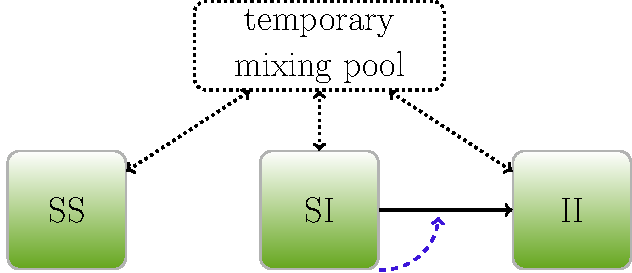
\includegraphics[width=0.9\linewidth]{tikz-f1}
  }
\caption{}
%\caption{Instantaneous switching without extra-pair contact (``instswitch'')}
\end{subfigure}
\begin{subfigure}[b]{0.4\linewidth}
	\centering
	  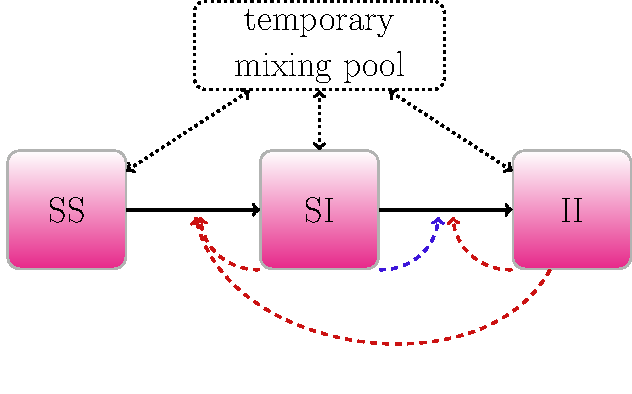
\includegraphics[width=0.9\linewidth]{tikz-f2}
\caption{}
%\caption{Instantaneous switching with extra-pair contact (``instswitch+epc'')}
\end{subfigure}

\begin{subfigure}[b]{0.4\linewidth}
	\centering
	\raisebox{0.33\height}{
	  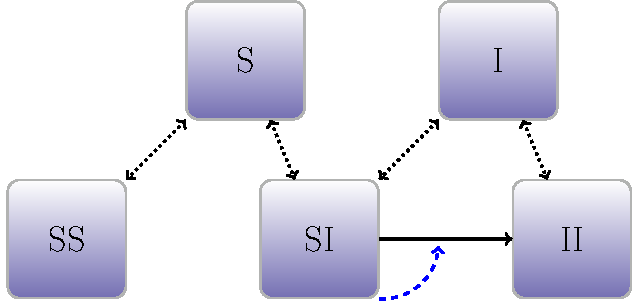
\includegraphics[width=0.9\linewidth]{tikz-f3}
	}
\caption{}
%\caption{Pair-formation model without extra-pair/uncoupled contact 
%(``pairform'')}
\end{subfigure}
\begin{subfigure}[b]{0.4\linewidth}
	\centering
	  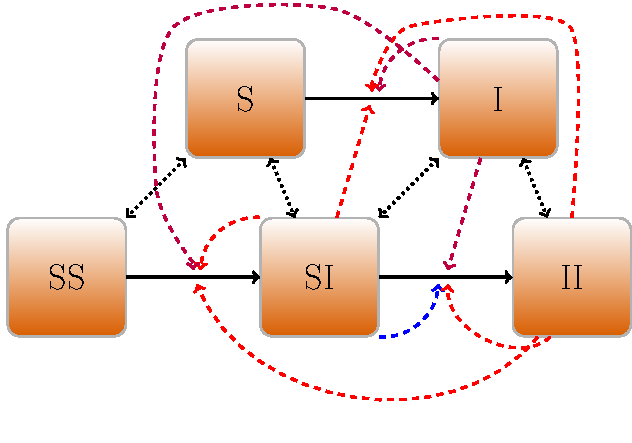
\includegraphics[width=0.9\linewidth]{tikz-f4}
\caption{}
%\caption{Pair-formation model with extra-pair/uncoupled contact
%(``pairform+epc'')}
\end{subfigure}
\end{figure}
\end{document}
